\documentclass[
aip,
jcp,
%preprint,
reprint,
]{revtex4-1}
%
\usepackage[hyperindex,breaklinks,hidelinks,colorlinks,citecolor=blue]{hyperref}
\usepackage{amsmath, amsthm, amssymb}    
\usepackage{float}
%
\usepackage{tabularx}
\newcolumntype{C}[1]{>{\centering\let\newline\\\arraybackslash\hspace{0pt}}m{#1}}
%
\usepackage{graphicx}
\DeclareGraphicsExtensions{.pdf,.eps,.png}
\graphicspath{{Figures/}}
\usepackage[outdir=Figures/]{epstopdf}
\newcommand{\figscale}{0.8}
%
\usepackage{natmove}
%
%\usepackage{mathtools}
%\mathtoolsset{showonlyrefs}
%
\DeclareMathOperator\arctanh{arctanh}
\DeclareMathOperator\arcsinh{arcsinh}
\DeclareMathOperator\sech{sech}
%
\newcommand{\mt}[1]{\boldsymbol{\mathbf{#1}}}          % matrix symbol
\newcommand{\vt}[1]{\boldsymbol{\mathbf{#1}}}          % vector symbol
\newcommand{\tr}[1]{#1^\text{t}}                       % transposition
\newcommand{\diff}[2]{\frac{\partial #2}{\partial #1}} % derivative
\newcommand{\avg}[1]{\overline{#1}}                    % average
\newcommand{\Liu}{\mathcal{L}}
\newcommand{\Ham}[1]{{\mathcal H}_\mathrm{#1}}         % Hamiltonian
%\newcommand{\grad}[2]{\nabla_{#1}{#2}}                 % gradient
\newcommand{\grad}[2]{\diff{#1}{#2}}                   % gradient

% Symbols:
\newcommand{\nn}{n}

% Temporary:
\usepackage{soul}

\begin{document}

\author{Charlles R. A. Abreu}
\email{abreu@eq.ufrj.br}
\affiliation{Chemical Engineering Department, Escola de Qu\'imica, Universidade Federal do Rio de Janeiro, Rio de Janeiro, RJ 21941-909, Brazil}
\affiliation{Department of Chemistry, New York University, New York, New York 10003, USA}

\author{Mark E. Tuckerman}
\email{marktuckerman@nyu.edu}
\affiliation{Department of Chemistry, New York University, New York, New York 10003, USA}
\affiliation{Courant Institute of Mathematical Sciences, New York University, New York, New York 10012, USA}
\affiliation{NYU-ECNU Center for Computational Chemistry at NYU Shanghai, Shanghai 200062, China}

\title{New Methods for Enabling Very Large Time Steps in Multiple Time-Scale Molecular Dynamics}

\keywords{molecular dynamics; multiple time-stepping; resonance}

\date{\today}

\maketitle

\section{Introduction}

Multiple time-scale (MTS) integration \cite{Grubmuller_1991, Tuckerman_1992, Martyna_1996} is an effective way of improving the efficiency of Molecular Dynamics (MD) simulations.
In classical MD, it allows the most expensive computations, such as the evaluation of long-range van der Waals and electrostatic components of a force field, to be done less frequently than others.
This is possible because the characteristic rates of variation of such contributions are much smaller than those of both non-bonded interactions at short distances and bonded intramolecular forces.
If estimating free-energy differences or other ensemble averages is the main goal of a simulation, then the maximum benefit one can get from multiple time-stepping occurs when it is possible to match the outermost step size with the correlation time of the system dynamics, i.e., the sampling period required to obtain a series of uncorrelated configurations.
Although this is theoretically feasible in many situations, it took long until the capacity of MTS integration could be fully realized.
The cause of such delay is the emergence of resonance artifacts \cite{Biesiadecki_1993, Schlick_1998a, Ma_2003} which limit the maximum attainable step size.

Attempts have been made over the years to overcome the mentioned limitation.
One of the strategies, known as mollified impulse \cite{Garcia-archilla_1998, Skeel_1999}, relies on altering the slow part of the potential energy function.
This is done by evaluating the corresponding forces at filtered positions, averaged along auxiliary trajectories which are, in turn, dictated by the fast part of the potential.
However, the most successful approach for dealing with resonance artifacts in constant-temperature MD does not involve altering the potential.
Instead, it entails introducing new dynamic variables (i.e.e an extended-system approach) and enforcing massive isokinetic constraints \cite{Minary_2003a, Minary_2003b, Minary_2004, Leimkuhler_2013}.
The basic recipe consists in pairing the velocity of each physical degree of freedom in the system with a set of extended-space velocities.
Then, individual thermostats are attached to all these extra velocities instead of the physical ones.
Finally, the combined kinetic energy of each set of physical and its corresponding extra velocities is enforced to be constant.
In this way, the magnitude of every velocity can never exceed a certain value and, consequently, the likelihood of resonance and instability in the simulated dynamics goes down significantly.
This procedure is clearly not meant to reproduce the Maxwell-Boltzmann distribution of velocities of a canonical ensemble, but it provides the correct distribution of coordinates \cite{Minary_2003a, Minary_2003b, Minary_2004, Leimkuhler_2013}.
The method was originally formulated \cite{Minary_2003a, Minary_2003b, Minary_2004} with deterministic thermostats \cite{Martyna_1992} and subsequently reformulated \cite{Leimkuhler_2013} with stochastic ones \cite{Samoletov_2007, Leimkuhler_2009}.

There is a rich literature on the development and analysis of extended-system methods \cite{Martyna_1996, Tuckerman_1999, Tuckerman_2001a, Sergi_2001, Ezra_2004, Tuckerman_2010}.
Pioneered in the 1980's \cite{Andersen_1980, Nose_1984, Hoover_1985}, they allowed the use of MD to study thermodynamic systems under the influence of external baths.
Nevertheless, the isokinetic formulation is somewhat extraneous in such universe.
Some of the well-established tools developed in the area are not readily applicable to its analysis.
As a consequence, knowledge about the properties of isokinetic methods has been advancing in a case-by-case basis.
Once this is the first approach that allows MTS simulations with very large time steps, it becomes particularly hard to distinguish the actual cause of observed anomalies.

In the present paper, we introduce a novel resonance-control methodology and demonstrate that it is completely equivalent to the isokinetic framework.
It consists in substituting the kinetic part of the system Hamiltonian by a new momentum-dependent function, whose main feature is also causing the confinement of velocities to a fixed range.
The potential part of the Hamiltonian is kept unchanged.
We are, thus, recasting the isokinetic approach is a form that is more akin to standard extended-system and stochastic methods.
This allowed us to unveil certain properties of the isokinetic dynamics which remained hitherto unnoticed, such as 1) the driven-variable nature of the extra velocities, 2) the existence of additional conserved quantities, and 3) some odd forms of velocity frequency distributions.
More importantly, it became straightforward to devise a new, Langevin-type version of the method with superior performance.

\section{Methods}
\label{sec:methods}

\subsection{Molecular Dynamics in the Canonical Ensemble}
\label{sec:standard canonical ensemble}

For a classical system with coordinates $\vt r$, we are often interested in obtaining canonical-ensemble averages of a purely configurational property, say,
\begin{equation*}
\label{eq:configurational average}
\langle A \rangle = \frac{1}{Z} \int e^{-\frac{U(\vt r)}{kT}} A(\vt r) d\vt r,
\end{equation*}
where $T$ is the temperature, $k$ is the Boltzmann constant, $U(\vt r)$ is a potential energy function, and $Z$ is a normalizing constant.
This is usually accomplished by defining a standard Hamiltonian $\mathcal{H}(\vt r, \vt p) = U(\vt r) + \sum_{i=1}^{N_f} \frac{p_i^2}{2 m_i}$ and exploring the phase space by means of some canonical (constant NVT) dynamics method.
In this expression, $p_i$ is the conjugate momentum and $m_i$ is the mass associated to a degree of freedom $i$, whose total number is $N_f$.
This procedure results in a probability density $\rho(\vt r, \vt p) \propto e^{-\frac{\mathcal{H}(\vt r, \vt p)}{kT}}$, up to small systematic deviations introduced by the numerical discretization of time \cite{Eastwood_2010, Davidchack_2010, Silveira_2017a, Silveira_2019a}.
As a result, coordinates are sampled with the desired probabilities and, at the same time, each momentum $p_i$ fluctuates according to a zero-mean normal distribution with standard deviation $\sigma_i = \sqrt{m_i k T}$.

In a Hamiltonian dynamics, as well as in most non-Hamiltonian methods devised to sample the canonical ensemble, the velocity of a particle is the gradient of $\mathcal{H}$ with respect to its momentum, that is,
\begin{equation}
\label{eq:velocity as momentum gradient}
v_i = \diff{p_i}{{\mathcal H}}.
\end{equation}

Therefore, in a simulation with the standard Hamiltonian, in which $v_i = \frac{p_i}{m_i}$, a large displacement will take place whenever the absolute value of some momentum increases excessively due to the action of a large force.
Time discretization can cause such forces to emerge due to, for instance, spurious atomic overlaps, thus causing numerical instability.
Massive isokinetic methods \cite{Minary_2003a, Minary_2003b, Minary_2004, Leimkuhler_2013} manage to avoid this problem by setting an upper bound to the kinetic energy of every degree of freedom.
Therefore, the largest single-step displacement that a coordinate $r_i$ can undergo during a massive isokinetic simulation is $c_i \delta t$, where $\delta t$ is the size of each time step -- or each inner time step, in the case of a MTS simulation -- and $c_i$ is the speed limit imposed to such degree of freedom (in allusion to the role that the speed of light plays in Special Relativity).
A side-effect of this strategy is that the probability distribution of velocities is no longer Gaussian, but has a particular form that depends on the number of thermostats attached to each degree of freedom \cite{Abreu_2020}.
On one hand, the details of the velocity and momentum distributions are not particularly relevant if one is only interested in configurational averages.
On the other hand, mixing time can actually be affected, thus altering the efficiency with which the coordinate space is sampled.
We have shown \cite{Abreu_2020} that, on average, each atom is slower in an isokinetic dynamics than it would be in a standard dynamics at the same temperature.

\subsection{New Hamiltonian for Regulated Isothermal Dynamics}
\label{sec:new hamiltonian}

Inspired by the massive isokinetic methods \cite{Minary_2003a, Minary_2003b, Minary_2004, Leimkuhler_2013}, we propose a new approach to impose a speed limit $c_i$ to every degree of freedom of a dynamical system.
This approach, which we will refer to as \textit{regulated dynamics}, consists in using a modified Hamiltonian, given by
\begin{equation}
\label{eq:modified hamiltonian}
\mathcal{H}_\nn(\vt r, \vt p) = U(\vt r) + \nn kT \sum_{i=1}^{N_f} \ln \cosh\left(\frac{p_i}{\sqrt{\nn m_i k T}}\right),
\end{equation}
where $\nn > 0$ is an arbitrary parameter.

The new Hamiltonian shares important properties with the standard one.
For instance, by being an even function of every $p_i$, it is invariant to momentum sign flips.
Moreover, it is separable with respect to the set of coordinates and to every individual momentum, which makes the marginal equilibrium distributions of $\vt r$ and $\vt p$ independent of each other, as well as those of $p_i$ and $p_j$ whenever $i \neq j$.
Together with the condition that $e^{-\frac{\mathcal{H}_\nn(\vt r, \vt p)}{k T}} \to 0$ when any $p_i \to \pm \infty$, such separability renders valid  \cite{Uline_2008} the generalized equipartition theorem \cite{Tolman_1918a}, which states that
\begin{equation}
\label{eq:generalized equipartition}
\left\langle v_i p_i \right\rangle = k T.
\end{equation}

Another desirable feature of $\mathcal{H}_\nn$ is that it approaches the standard Hamiltonian when $\nn$ increases.
This becomes clear by observing the Taylor series expansion
\begin{equation*}
\nn \ln \cosh\left(\frac{x}{\sqrt{\nn}}\right) = \frac{x^2}{2} - \frac{x^4}{12 \nn} + \frac{x^6}{45 \nn^2} + \mathcal{O}(x^8).
\end{equation*}

If a constant-NVT simulation is set up with the new Hamiltonian, coordinates will still be sampled proportionally to $e^{-\frac{U(\vt r)}{kT}}$, as it was designed to do, while each momentum $p_i$ will be sampled according to a probability density given by
\begin{equation}
\label{eq:momentum distribution}
\rho_\nn(p_i) = \frac{\Gamma\left(\frac{\nn+1}{2}\right)}{\Gamma\left(\frac{\nn}{2}\right) \sqrt{\pi \nn m_i k T}} \sech^\nn\left(\frac{p_i}{\sqrt{\nn m_i k T}}\right),
\end{equation}
where $\Gamma$ is the complete gamma function.
This probability density, whose normalization constant is obtained in Appendix \ref{sec:momentum and velocity distributions}, is depicted in the top row of Fig.~\ref{fig:momentum and velocity functions} for various integer values of $\nn$.
The tendency towards the normal distribution with increasing $\nn$ is evident.
The figure also depicts, in the middle row, the relation between velocity and momentum for the same values of $\nn$.
Such relation, obtained from Eqs.~\eqref{eq:velocity as momentum gradient} and \eqref{eq:modified hamiltonian}, is
\begin{equation}
	\label{eq:velocity definition}
	v_i = c_i \tanh\left(\frac{p_i}{m_i c_i}\right),
\end{equation}
	where the speed limit $c_i$ is given by
\begin{equation}
	\label{eq:speed limit definition}
	c_i = \sqrt{\frac{\nn k T}{m_i}}.
\end{equation}

\begin{figure}[htbp!]
	\centering
	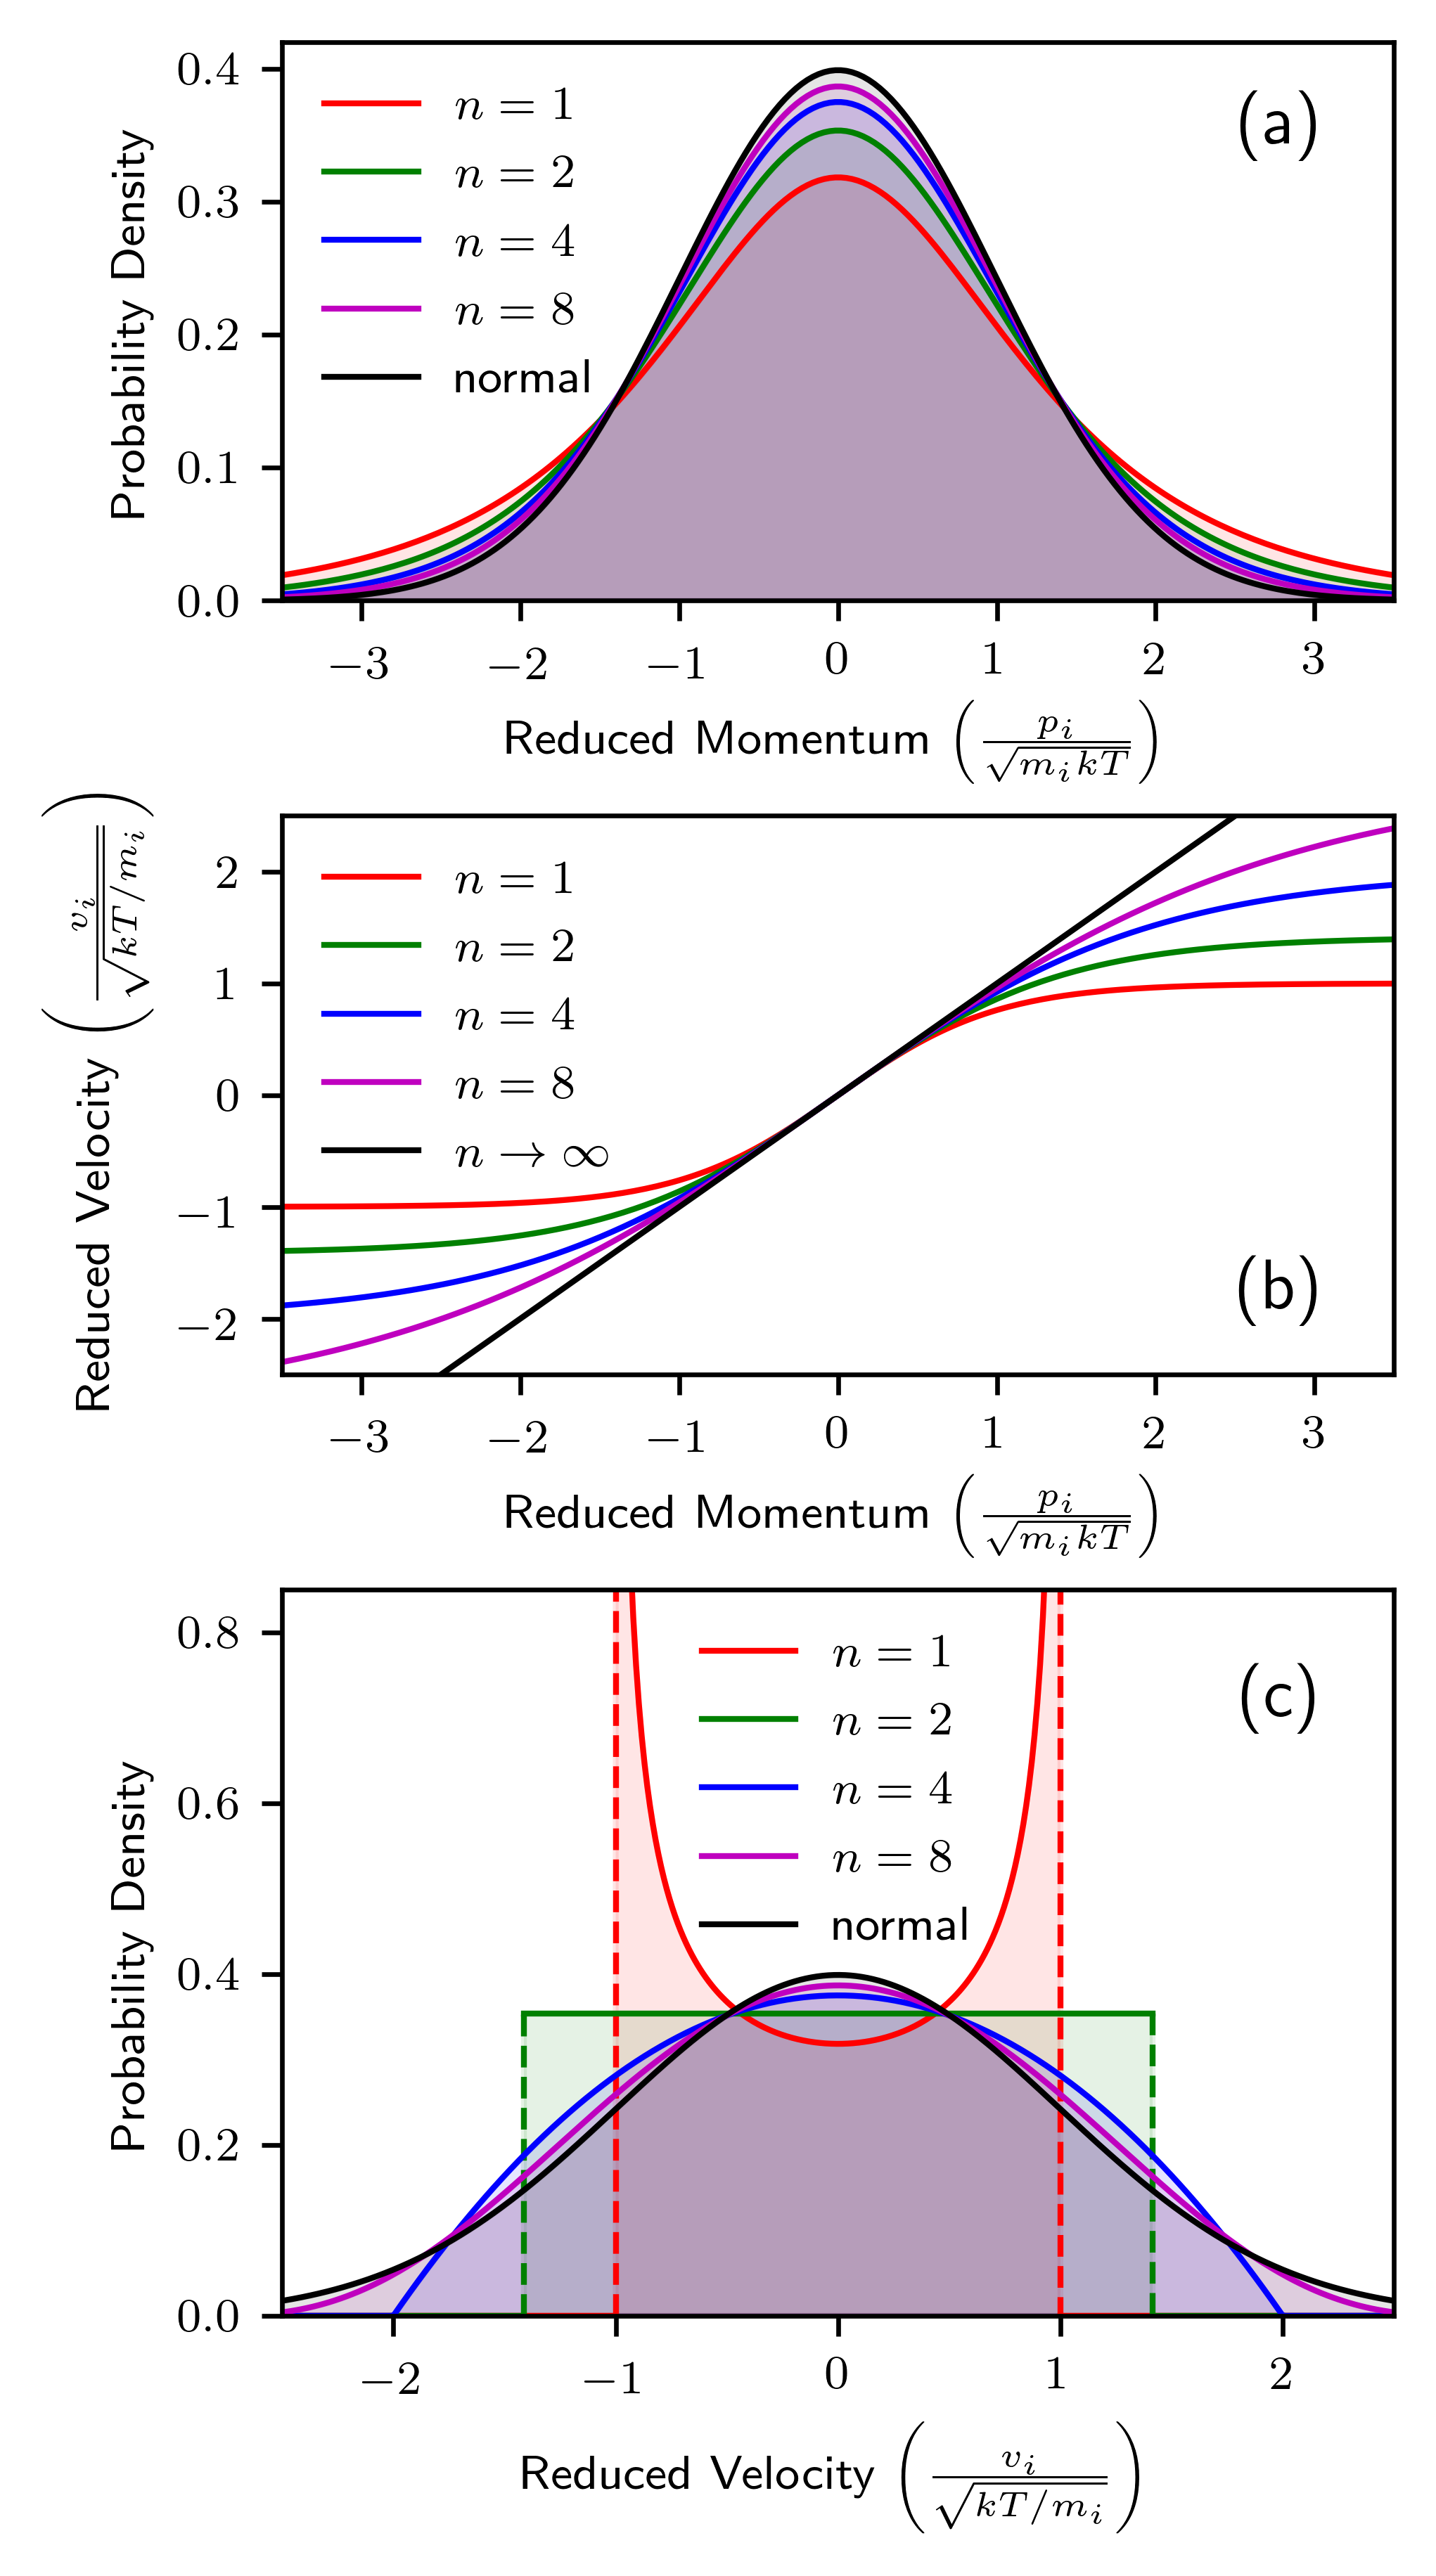
\includegraphics[scale=\figscale]{momentum_and_velocity_functions}
	\caption{Momentum distributions (top) and velocities (bottom)}
	\label{fig:momentum and velocity functions}
\end{figure}

It is interesting to observe the distribution of velocities, whose PDF is derived in Appendix \ref{sec:momentum and velocity distributions} and is given by
\begin{equation*}
\varrho_\nn(v_i) = \begin{cases}
\frac{1}{c_i} \frac{\Gamma\left(\frac{\nn+1}{2}\right)}{\Gamma\left(\frac{\nn}{2}\right) \sqrt{\pi}} \left(1-\frac{v_i^2}{c_i^2}\right)^{\frac{\nn}{2}-1} & \mathrm{if} \; v_i^2 \leq c_i^2 \\
0 & \mathrm{otherwise}
\end{cases}.
\end{equation*}

This is depicted in the bottom row of Fig.~\ref{fig:momentum and velocity functions} for the same values of $\nn$ employed before.
With $\nn \in \mathbb{N}$, such distribution becomes identical to the one corresponding to the massive isokinetic dynamics \cite{Abreu_2020}, with parameter $\nn$ substituting the number of thermostats attached to each degree of freedom.
One important aspect of this distribution, which will be essential in the forthcoming discussion about thermostat algorithms, is the special form of the kinetic energy equipartition it implies (see Appendix~\ref{sec:momentum and velocity distributions}), given by
\begin{equation}
\label{eq:special kinetic energy equipartition}
\left\langle m_i v_i^2 \right\rangle = \frac{\nn}{\nn+1} kT.
\end{equation}

The standard canonical-ensemble equipartition is approached only if $\nn$ is large.
Such approach comes from below, meaning that particles are slower, on average, than their counterparts in a canonical ensemble at the same temperature.
We have already observed this fact in the case of massive isokinetic dynamics methods \cite{Abreu_2020}, with implications in their capability of producing uncorrelated samples for configurational property inference.
With a single thermostat per degree of freedom, for instance, the mean kinetic energy of the system is only half the value corresponding to a standard canonical ensemble.
Following the same principle, it is straightforward to devise a Hamiltonian that would lead to the standard equipartition equation regardless of the value of $\nn$.
It is
\begin{equation*}
\mathcal{H}^\mathrm{eq}_\nn(\vt r, \vt p) = U(\vt r) + \nn kT \sum_{i=1}^{N_f} \ln \cosh\left(\sqrt{\frac{\nn+1}{\nn^2 m_i k T}} p_i\right).
\end{equation*}

However, as we show in this article through numerical tests (see Sec.~\ref{sec:liquid water simulations}), such alternative Hamiltonian brings about new artifacts that impair its performance in multiple time-scale simulations when compared to that obtained from using Eq.~\eqref{eq:modified hamiltonian}.
The reason becomes clear if contrast Fig.~\ref{fig:momentum and velocity functions}(b) with Fig.~\ref{fig:alternative velocity functions}, which shows the velocity-momentum relation that results from $\mathcal{H}^\mathrm{eq}_\nn$.
In Fig.~\ref{fig:momentum and velocity functions}(b), all curves collapse towards the diagonal line around $p_i = 0$.
This is where the peak of the momentum distribution is, meaning that particles will most likely move in nearly the same direction of their momentum vectors, which are in turn guided by the resultant forces acting on them.
This resembles the dynamics of a canonical ensemble, with only fast particles deviating from the force-dictated directions as a way to comply with the imposed speed limit.
In contrast, Fig.~\ref{fig:alternative velocity functions} shows that the price for making the standard equipartition equation valid even for small $\nn$ values is that velocities will always diverge from the force-induced directions.

\begin{figure}[htbp!]
	\centering
	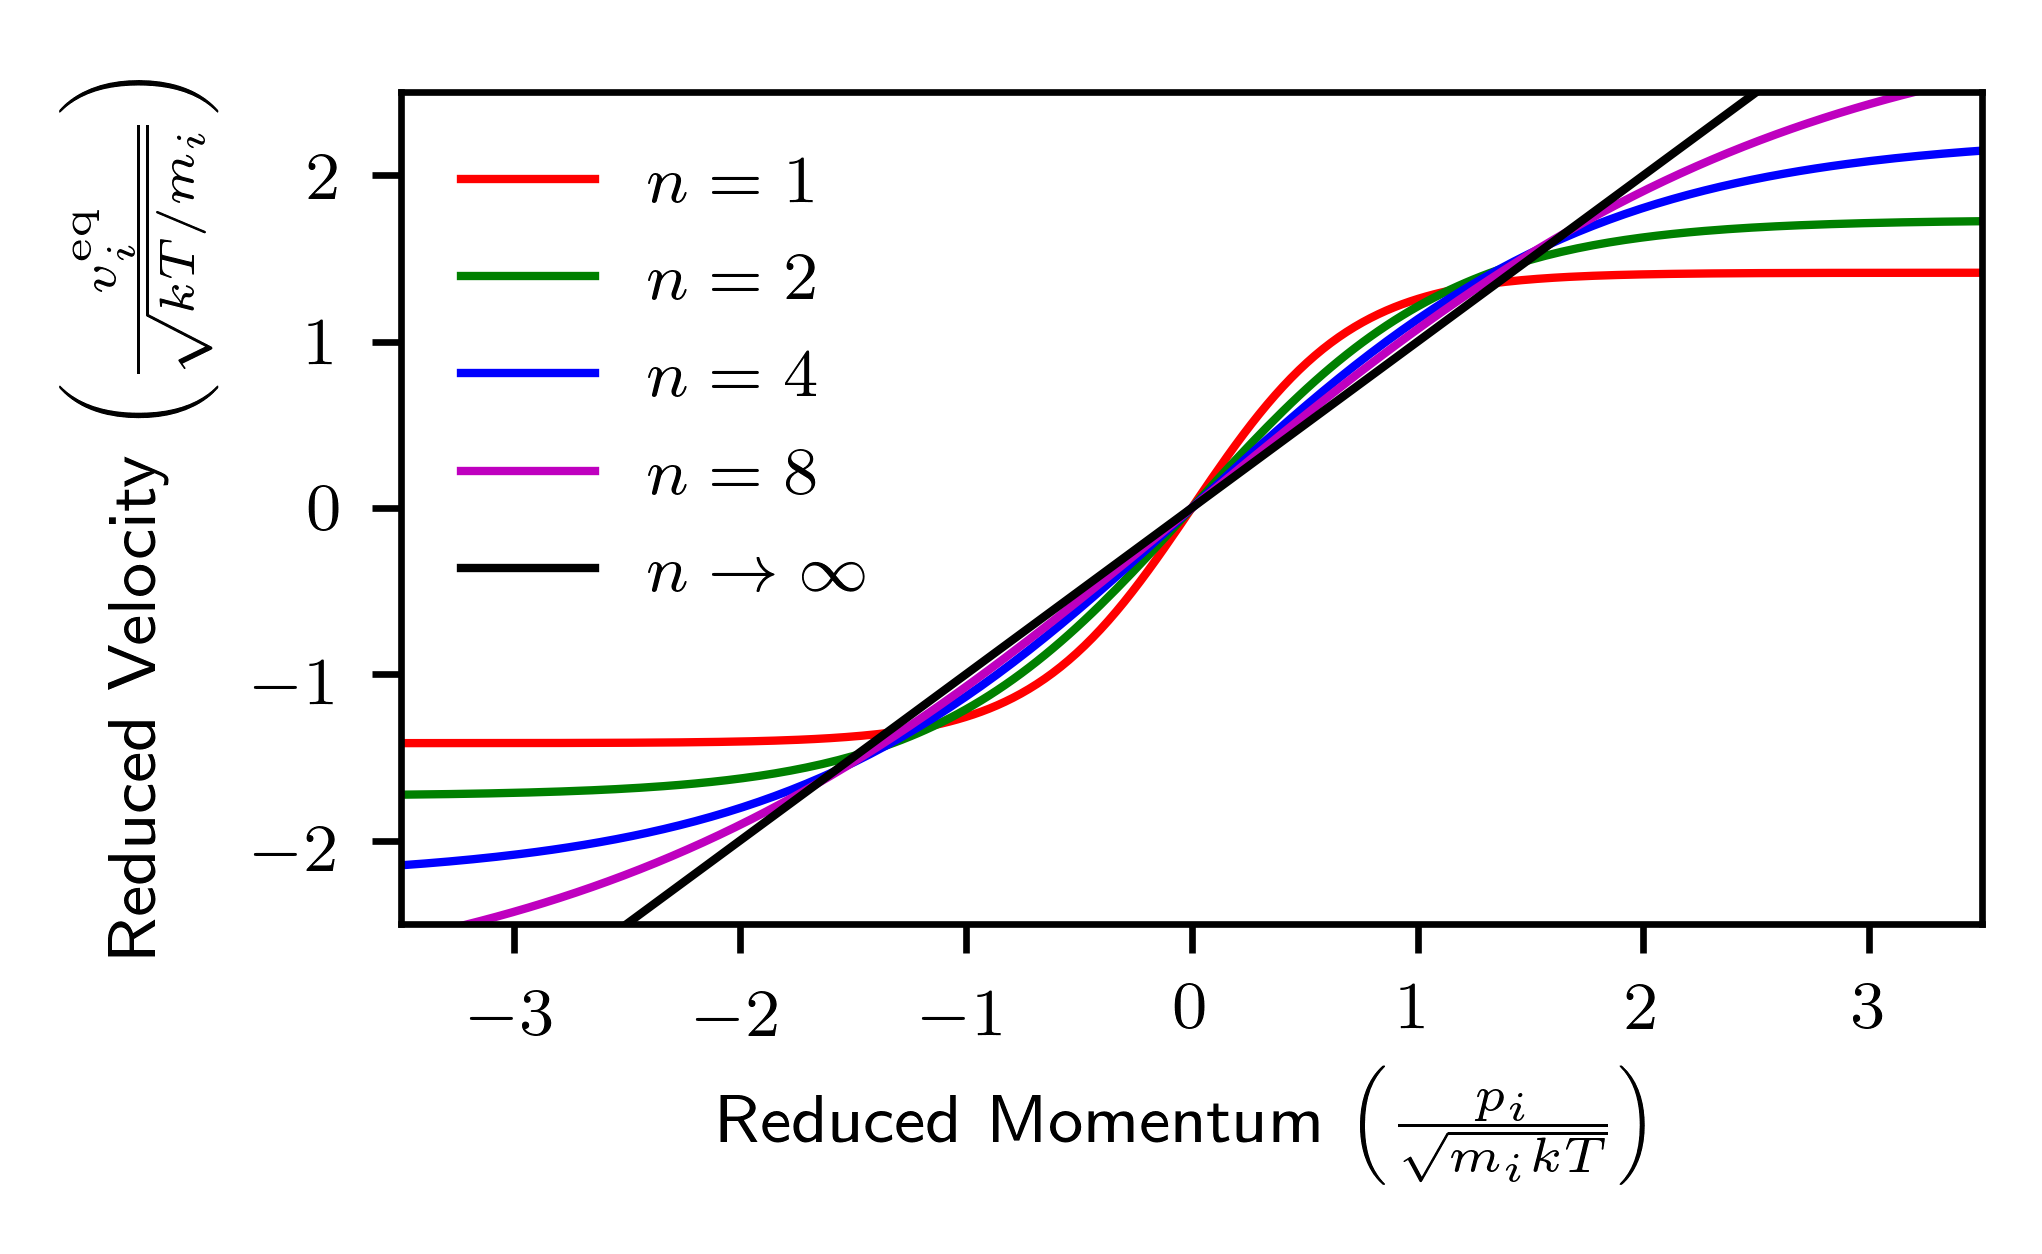
\includegraphics[scale=\figscale]{alternative_velocity_functions}
	\caption{Momentum distributions (top) and velocities (bottom)}
	\label{fig:alternative velocity functions}
\end{figure}

In the forthcoming sections, we deal with simulation methods that aim at reproducing a canonical distribution with the new Hamiltonian.
First, we employ a massive version of an existing thermostat algorithm and show that it simply relies on the validity of the generalized equipartition theorem, Eq.~\eqref{eq:generalized equipartition}, in order to enact correct thermostatting.
Next, we devise a new algorithm which relies on the especial equipartition given by Eq.~\eqref{eq:special kinetic energy equipartition} instead.
A marked difference between these two principles is that the quantity subject to equipartition in Eq.~\eqref{eq:generalized equipartition} is unbounded due to the presence of $p_i$, whereas its counterpart in Eq.~\eqref{eq:special kinetic energy equipartition} has $m_i c_i^2$ an upper bound.
For this reason, we will classify methods based on the former equation as semi-regulated, as a way of distinguishing them from those based on the latter.
Finally, although this is beyond the scope of this article, it is worth mentioning that higher-order central moments (see Appendix~\ref{sec:momentum and velocity distributions}) can also be used for enacting thermostatting, such as in the Generalized Gaussian Moment algorithm \cite{Liu_2000}.

\subsection{Semi-Regulated Nos\'{e}-Hoover-Langevin Dynamics}
\label{sec:semi-regulated massive NHL thermostatting}

In order to derive equations of motion for a regulated NVT dynamics in the space of coordinates $\vt r$ and momenta $\vt p$, referred to hereafter as the physical phase space, we employ a massive version of the Nos\'{e}-Hoover-Langevin (NHL) method \cite{Samoletov_2007, Leimkuhler_2009}.
This begins by extending the phase space with $N_f$ extra pairs of coordinates $\vt \eta$ and conjugate momenta $\vt p_\eta$.
An inertial parameter $Q_i$ is associated to every degree of freedom.
The dynamics of the NHL method is described by a system of stochastic differential equations (SDE) expressed as
\begin{subequations}
	\label{eq:regulated massive NHL equations}
	\begin{align}
	&dr_i = v_i dt, \\
	&dp_i = \left(F_i - \frac{p_{\eta_i}}{Q_i} p_i\right) dt, \quad \mathrm{and} \\
	&dp_{\eta_i} = (p_i v_i - kT) dt - \gamma p_{\eta_i} dt + \sqrt{2 \gamma Q_i kT} dW_i,
	\end{align}
\end{subequations}
where $F_i = -\diff{r_i}{U}$ is the force exerted on $i$,
$\gamma$ is a friction constant, and
$dW_i$ denotes an infinitesimal increment of a Wiener process.
Each velocity $v_i$ is computed via Eq.~\eqref{eq:velocity definition}, which is the single difference between the regulated and standard versions of the massive NHL method.
An equation $d\eta_i = \frac{p_{\eta_i}}{Q_i} dt$ for each $i$ could have been included as well, but it can be ignored in practice for having no influence on the physical-space dynamics.
Nevertheless, it is important from a theoretical standpoint when it comes to demonstrating that such space is correctly sampled in accordance with $e^{-\frac{\mathcal{H}_\nn(\vt r, \vt p)}{kT}}$.

Although the main advantage of the proposed method shows up in the context of multiple time-scale simulations, we begin by presenting a single time-scale integration scheme, which can be easily extended afterwards.
As it has been demonstrated in recent years \cite{Leimkuhler_2013b, Zhang_2017, Li_2017, Fass_2018, Zhang_2019}, middle-type integration schemes are very accurate at reproducing the distribution of coordinates, at the expense of the distribution of velocities.
This is particularly appealing for the present method, given its pursued characteristics.
In the usual operator splitting notation, the time steps of our proposed middle-scheme integrator is \cite{Zhang_2017}
\begin{subequations}
\label{eq:single time scale integrator}
\begin{equation}
\label{eq:middle-type integrator}
e^{\delta t\Liu} = e^{\frac{\delta t}{2} \Liu^\mathrm{tr}_p} e^{\frac{\delta t}{2} \Liu^\mathrm{tr}_r} e^{\delta t\Liu_\mathrm{bath}} e^{\frac{\delta t}{2} \Liu^\mathrm{tr}_r} e^{\frac{\delta t}{2} \Liu^\mathrm{tr}_p},
\end{equation}
where
\begin{equation}
\label{eq:bath propagator}
e^{\delta t\Liu_\mathrm{bath}} = e^{\frac{\delta t}{2} \Liu^\mathrm{tr}_{p_\eta}} e^{\frac{\delta t}{2} \Liu^\mathrm{sc}_p} e^{\delta t \Liu^\mathrm{ou}_{p_\eta}} e^{\frac{\delta t}{2} \Liu^\mathrm{sc}_p} e^{\frac{\delta t}{2} \Liu^\mathrm{tr}_{p_\eta}}.
\end{equation}
\end{subequations}

In the propagators above, superscript `tr' stands for translation, meaning that the effects of propagators $e^{t \Liu^\mathrm{tr}_r}$, $e^{t \Liu^\mathrm{tr}_p}$, and $e^{t \Liu^\mathrm{tr}_{p_\eta}}$ on each degree of freedom $i$ can be expressed, respectively, as
\begin{align}
&r_i = r_i^0 + v_i^0 t, \label{eq:NHL move} \\
&p_i = p_i^0 + F_i^0 t, \quad \mathrm{and}  \\
&p_{\eta_i} = p_{\eta_i}^0 + (p_i^0 v_i^0 - kT) t,
\end{align}
where $v_i^0 = c_i \tanh\big(\frac{p_i^0}{m_i c_i}\big)$, whereas superscript $0$ denotes the initial condition encountered by a propagator and $t$ corresponds to the time span of its action.
In turn, superscript `sc' means scaling, so that $e^{t \Liu^\mathrm{sc}_p}$ is a propagator whose action on each momentum $p_i$ is
\begin{equation}
p_i = p_i^0 e^{-\frac{p_{\eta_i}^0}{Q_i} t}.
\end{equation}

Finally, `ou' refers to an Ornstein-Uhlenbeck stochastic process, so that the action of $e^{t \Liu^\mathrm{ou}_{p_\eta}}$ on each thermostat momentum $p_{\eta_i}$ can be executed as
\begin{equation}
p_{\eta_i} = p_{\eta_i}^0 e^{-\gamma t} + \sqrt{Q_i kT (1 - e^{-2\gamma t})} \xi_i,
\end{equation}
where $\xi_i$ is an independent random variate following the standard normal probability distribution.
Implementing the described propagators is straightforward once a computer code is available for evaluating the forces at every time step.

As done in Ref.~\citenum{Leimkuhler_2013}, we show that the Boltzmann-Gibbs distribution of coordinates is correctly obtained.
For this purpose, we derive the equilibrium distribution of the method in its deterministic limit, with $\gamma=0$.
After that, we show that the stochastic contribution keeps such distribution invariant.
The deterministic version of Eq.~\eqref{eq:regulated massive NHL equations} is a massive Nos\'e-Hoover \cite{Nose_1984, Hoover_1985} thermostat applied to $\mathcal{H}_\nn$ as expressed in Eq.~\eqref{eq:modified hamiltonian}.
It is a non-Hamiltonian dynamics that conserves an energy function defined as
\begin{equation}
\label{eq:extended energy}
H_\nn(\vt r, \vt p, \vt \eta, \vt p_\eta) = {\mathcal H}_\nn(\vt r, \vt p) + \sum_{i=1}^{N_f} \left(k T \eta_i + \frac{p_{\eta_i}^2}{2 Q_i} \right).
\end{equation}

A family of equations of motion devised to preserve $H_\nn$ can be written in the general form \cite{Sergi_2001}
\begin{equation}
\label{eq:general conservative phase-space flow}
\dot{\vt x} = {\mt B} \grad{\vt x}{H_\nn},
\end{equation}
where $\vt x$ is the vector of all extended phase-space variables, $\mt B$ is a skew-symmetric, matrix-valued function of $\vt x$, and $\grad{\vt x}{}$ is the gradient operator.
By virtue of the chain rule, the time derivative of any scalar function $f(\vt x)$ is given by $\dot f = \tr{\dot{\vt x}}\grad{\vt x}{f} = \tr{(\grad{\vt x}{H_\nn})} \tr{\mt B} (\grad{\vt x}{f})$.
This is a quadratic form, which becomes identically null whenever its defining matrix is skew-symmetric.
Hence, $\dot{H}_\nn = 0$.
For a massive thermostatting approach, both $\mt B$ and $\grad{\vt x}{H_\nn}$ can be organized blockwisely, with $\mt B$ having a block-diagonal structure.
In the case of a Nos\'e-Hoover dynamics, the blocks defined for each degree of freedom $i$ will be
\begin{equation}
\label{eq:regulated dynamics diagonal block}
{\mt B}_{i,i} =
\left[\begin{array}{cccc}
	0  &  1  & 0  &  0   \\
	-1 &  0  & 0  & -p_i \\
	0  &  0  & 0  &  1   \\
	0  & p_i & -1 &  0
\end{array}\right]
\quad \mathrm{and} \quad
\grad{\vt x_i}{H_\nn} =
\left[\begin{array}{c}
	         -F_i          \\
	         v_i           \\
	         k T           \\
	\frac{p_{\eta,i}}{Q_i}
\end{array}\right].
\end{equation}

Note that the entries of $\grad{\vt x_i}{H_\nn}$ are the derivatives of ${H_\nn}$ with respect to $r_i$, $p_i$, $\eta_i$, and $p_{\eta_i}$, respectively.
The present development will prove useful again in Sec.~\ref{sec:regulated massive NHL thermostatting}, where we derive a different method which also preserves $H_\nn$.
Now, it follows from Eqs.~\eqref{eq:general conservative phase-space flow} and \eqref{eq:regulated dynamics diagonal block} that
\begin{subequations}
	\label{eq:massive Nose-Hoover equations}
	\begin{align}
	&\dot{r}_i = v_i, \\
	&\dot{p}_i = F_i - \frac{p_{\eta_i}}{Q_i} p_i, \\
	&\dot{\eta}_i = \frac{p_{\eta_i}}{Q_i}, \quad \mathrm{and} \\
	&\dot{p}_{\eta_i} = v_i p_i - kT, \label{eq:massive Nose-Hoover p_eta}
	\end{align}
\end{subequations}
which is an ODE system that matches Eqs.~\eqref{eq:regulated massive NHL equations} in the deterministic limit.
By contrasting Eq.~\eqref{eq:massive Nose-Hoover p_eta} to Eq.~\eqref{eq:generalized equipartition}, we realize that described method has its base on the generalized equipartition theorem.

In order to apply the phase-space analysis method developed in Refs.~\citenum{Tuckerman_1999} and \citenum{Tuckerman_2001a}, we need to determine the phase space compressibility, which is defined as
\begin{equation}
\label{eq:phase space compressibility}
\kappa = \nabla_{\vt x} \cdot \dot{\vt x}.
\end{equation}

In the case of Eq.~\eqref{eq:massive Nose-Hoover equations},
\begin{equation}
\label{eq:Nose-Hoover compressibility}
\kappa = -\sum_{i=1}^{N_f} \frac{p_{\eta_i}}{Q_i} = -\sum_{i=1}^{N_f} \dot{\eta}_i.
\end{equation}

A phase-space flow like Eq.~\eqref{eq:general conservative phase-space flow} takes place in a manifold $H_\nn(\vt x) = H_\nn^0$, where the constant $H_\nn^0$ depends on the initial condition.
If this dynamics is ergodic and $H_\nn$ is the only conserved quantity, then the partition function of the resulting ensemble can be expressed as \cite{Tuckerman_1999, Tuckerman_2001a}
\begin{equation}
\label{eq:partition function definition}
\Omega = C \int \delta\Big(H_\nn(\vt x) - H_\nn^0\Big) \sqrt{g} d{\vt x},
\end{equation}
where $\delta(\cdot)$ is the Dirac delta function,
$\sqrt{g}$ is a metric determinant, and
$C$ is the proper statistical-mechanical prefactor, whose form is irrelevant for the present analysis.
For a system with internal forces only, Eq.~\eqref{eq:massive Nose-Hoover equations} also preserves quantities related to the sum of all momenta at each spatial dimension.
However, we can ignore these conservation laws here as we will eventually include a stochastic component to the equations of motion.
This way, according to Refs.~\citenum{Tuckerman_1999} and \citenum{Tuckerman_2001a}, we must simply substitute $e^{-w}$ for $\sqrt{g}$ in Eq.~\eqref{eq:partition function definition}, where $w$ is defined so that $\dot{w} = \kappa$ \cite{Tuckerman_1999, Tuckerman_2001a}.
Therefore, it follows from Eq.~\eqref{eq:Nose-Hoover compressibility} that
\begin{multline}
\label{eq:partition function result}
\Omega = C \int \delta\Big(H_\nn(\vt x) - H_\nn^0\Big) e^{\sum_{i=1}^{N_f} \eta_i} d{\vt x} = \\
= \frac{C e^{-\frac{H_\nn^0}{kT}}}{kT} \int e^{-\frac{\mathcal{H}_\nn(\vt r, \vt p) + \frac{1}{2 Q_i} \|{\vt p}_\eta\|^2}{kT}} d{\vt r} d{\vt p} d{\vt p}_\eta,
\end{multline}
where integration has been carried out for all $\eta_i$ after replacing $H_\nn(\vt x)$ from Eq.~\eqref{eq:extended energy}.
This result shows that the marginal distribution in the physical phase space will be proportional to $e^{-\frac{\mathcal{H}_\nn(\vt r, \vt p)}{kT}}$.
In addition, each extended-space momentum $p_{\eta_i}$ follows a normal distribution with variance $\sigma_i^2 = Q_i k T$.
As shown in Ref.~\citenum{Leimkuhler_2013} by means of the Fokker-Planck equation, the latter condition is sufficient for the complete set of stochastic equations of motion to maintain the limiting distribution implied by the partition function above.

\subsection{Regulated Nos\'{e}-Hoover-Langevin Dynamics}
\label{sec:regulated massive NHL thermostatting}

We now propose a different version of the massive NHL algorithm, whose thermostatting capability relies on the special form of the kinetic energy equipartition expressed in Eq.~\eqref{eq:special kinetic energy equipartition}.
Based on the developments of Sec.~\ref{sec:semi-regulated massive NHL thermostatting}, we begin by describing the deterministic version of the method before including a Langevin-type thermostat.
The new equations of motion can be obtained by simply modifying some entries of the matrix $\mt B$, which is present in Eqs.~\eqref{eq:general conservative phase-space flow} and \eqref{eq:regulated dynamics diagonal block}, while maintaining its skew-symmetric and block-diagonal structures.
Each block in the main diagonal of the modified matrix is
\begin{equation}
{\mt B}_{i,i} =
\left[
\begin{array}{cccc}
	0  &    1    &           0           &           0           \\
	-1 &    0    &           0           &       -m_i v_i        \\
	0  &    0    &           0           & 1-\frac{v_i^2}{c_i^2} \\
	0  & m_i v_i & \frac{v_i^2}{c_i^2}-1 &           0
\end{array}
\right].
\end{equation}

As a result, Eq.~\eqref{eq:general conservative phase-space flow} becomes
\begin{subequations}
	\label{eq:modified massive Nose-Hoover equations}
	\begin{align}
	&\dot{r}_i = v_i, \\
	&\dot{p}_i = F_i - \frac{p_{\eta_i}}{Q_i} m_i v_i,  \label{eq:modified massive Nose-Hoover p} \\
	&\dot{\eta}_i = \left(1 - \frac{v_i^2}{c_i^2}\right) \frac{p_{\eta_i}}{Q_i}, \quad \mathrm{and} \\
	&\dot{p}_{\eta_i} = \frac{\nn+1}{\nn} m_i v_i^2 - kT \label{eq:modified massive Nose-Hoover p_eta}.
	\end{align}
\end{subequations}

We should now contrast Eq.~\eqref{eq:modified massive Nose-Hoover p_eta} to Eq.~\eqref{eq:special kinetic energy equipartition}.
Due to the skew symmetry of $\mt B$, it is straightforward to conclude that the equations above preserve the extended energy defined in Eq.~\eqref{eq:extended energy}.
The phase-space compressibility they imply is $\kappa = - \sum_{i=1}^{N_f} \frac{p_{\eta_i}}{Q_i} m_i \frac{d v_i}{d p_i}$.
From Eq.~\eqref{eq:velocity definition}, it follows that
\begin{equation}
\label{eq:velocity derivative wrt momentum}
\frac{d v_i}{d p_i} = \frac{1}{m_i} \left[1 - \tanh^2\left(\frac{p_i}{m_i c_i}\right)\right] = \frac{1}{m_i} \left(1 - \frac{v_i^2}{c_i^2}\right).
\end{equation}

Therefore,
\begin{equation}
\kappa = - \sum_{i=1}^{N_f} \frac{p_{\eta_i}}{Q_i} \left(1 - \frac{v_i^2}{c_i^2}\right) = -\sum_{i=1}^{N_f} \dot{\eta}_i.
\end{equation}

Remarkably, this result guarantees that the modified method will produce the same partition function shown in Eq.~\eqref{eq:partition function result} and, therefore, the same limiting distribution in the physical phase space.
We are now ready to include the stochastic contributions to the equations of motion, which then become
\begin{subequations}
	\label{eq:modified massive Nose-Hoover-Langevin equations}
	\begin{align}
	&dr_i = v_i dt, \\
	&dp_i = \left(F_i - \frac{p_{\eta_i}}{Q_i} m_i v_i\right) dt, \quad \mathrm{and} \\
	&dp_{\eta_i} = \left(\frac{\nn+1}{\nn} m_i v_i^2 - kT\right) dt \nonumber \\
	& \qquad \qquad \qquad - \gamma p_{\eta_i} dt + \sqrt{2 \gamma Q_i kT} dW_i \label{eq:modified massive Nose-Hoover-Langevin p_eta}.
	\end{align}
\end{subequations}

Here we have, once again, omitted the decoupled equation of motion of each variable $\eta_i$.
Numerical integration of this new system of equations can be done similarly to that of Eqs.~\eqref{eq:regulated massive NHL equations}, with only two differences.
The first one lies in the action of the translation propagator $e^{t \Liu^\mathrm{tr}_{p_\eta}}$, which is now expressed as
\begin{equation*}
p_{\eta_i} = p_{\eta_i}^0 + \left[\frac{\nn+1}{\nn} m_i (v_i^0)^2 - kT\right] t.
\end{equation*}

The second difference lies in the evaluation of the scaling propagator $e^{t \Liu^\mathrm{sc}_p}$, whose action consisting in the analytical solution of the differential equation
\begin{equation*}
\dot{p}_i = -v_{\eta_i} m_i v_i = -v_{\eta_i} m_i c_i \tanh\left(\frac{p_i}{m_i c_i}\right).
\end{equation*}

By changing variables from $p_i$ to $y_i = \sinh(\frac{p_i}{m_i c_i})$,
%so that $\dot{y}_i = \cosh(\frac{p_i}{m_i c_i}) \frac{\dot{p}_i}{m_i c_i}$,
the differential equation above becomes $\dot{y}_i = -v_{\eta_i} y_i$, whose solution is the simple scaling $y_i = y_i^0 e^{-v_{\eta_i} t}$.
Therefore, by changing back from $y_i$ to $p_i$, the action of $e^{t \Liu^\mathrm{sc}_p}$ becomes
\begin{equation*}
p_i = m_i c_i \arcsinh\left[\sinh\left(\frac{p_i^0}{m_i c_i}\right)e^{-v_{\eta_i}^0 t}\right].
\end{equation*}

With these two propagators having their new meanings, a single time-scale integration step can again be designed in a middle type of scheme as in Eq.~\eqref{eq:single time scale integrator}.

\subsection{Close Connection to Massive Isokinetic Dynamics}
\label{sec:modified NHC thermostatting}

As we mentioned in Sec.~\ref{sec:new hamiltonian}, a special case of our proposed Hamiltonian, namely when $n \in \mathbb{N}$, generates a canonical ensemble whose velocity distribution equals that of an isokinetic ensemble \cite{Abreu_2020} with $\nn$ thermostats per degree of freedom.
This already attests a close relationship between the two methodologies.
In the present section, we go further to demonstrate that our second proposed set of equations of motion, the one based on the special equipartition relation in Eq.~\eqref{eq:special kinetic energy equipartition}, produces also the same dynamics as the Stochastic Isokinetic Nos\'e-Hoover method \cite{Leimkuhler_2013} when $\nn = 1$.

First, we eliminate $p_i$ from Eq.~\eqref{eq:modified massive Nose-Hoover p} by resorting to Eqs.~\eqref{eq:speed limit definition} and \eqref{eq:velocity derivative wrt momentum}, from which we deduce that
\begin{equation}
\label{eq:velocity equation}
\dot{v}_i = \frac{dp_i}{dv_i} \dot{p}_i = \left(1 - \frac{m_i v_i^2}{\nn k T}\right) \left(\frac{F_i}{m_i} - v_{\eta_i} v_i\right).
\end{equation}

Next, we define a new variable $v_{1,i}$ and a new equation of motion for each degree of freedom $i$, which is
\begin{equation}
\label{eq:new driven variable equation}
\dot{v}_{1,i} = -\frac{F_i v_i - \frac{p_{\eta_i}}{Q_i} m_i v_i^2}{\nn kT} v_{1,i}.
\end{equation}

Note that this new equation does not alter the dynamics of the preexisting variables, meaning that each $v_{1,i}$ is a driven variable \cite{Tuckerman_1999, Tuckerman_2001a}.
Moreover, if $v_{1,i}(0) = 0$, it will remain null permanently.
Otherwise, it will vary in time but never change signs, since its rate of change vanishes when its own value approaches zero.
We now show that the same features are shared by a variable $\Phi_i$ defined as
\begin{equation}
\label{eq:isokinetic variable equation}
\Phi_i = m_i v_i^2 + \frac{\nn}{\nn+1} Q_1 v_{1,i}^2 - \nn k T,
\end{equation}
whose rate of change is $\dot{\Phi}_i = 2 (m_i v_i \dot{v}_i + \frac{\nn}{\nn+1} Q_1 v_{1,i} \dot{u}_i)$.
From Eqs.~\eqref{eq:velocity equation}-\eqref{eq:isokinetic variable equation}, it turns out that
\begin{equation*}
\dot{\Phi}_i = - 2 \frac{F_i v_i - \frac{p_{\eta_i}}{Q_i} m_i v_i^2}{\nn k T} \Phi_i,
\end{equation*}
which has nearly the same form as Eq.~\eqref{eq:isokinetic variable equation}.
Therefore, if an initial condition is assigned for all $v_{1,i}$ so that $\Phi_i(0) = 0$, then the dynamics will proceed in such a way that, at all times, it satisfies
\begin{equation}
\label{eq:isokinetic condition}
m_i v_i^2 + \frac{\nn}{\nn+1} Q_1 v_{1,i}^2 = \nn k T.
\end{equation}

The equation above is an isokinetic condition.
It is not a constraint, once $v_{1,i}$ is not a true dynamical variable in our approach.
Moreover, we can rewrite Eqs.~\eqref{eq:velocity equation} and \eqref{eq:new driven variable equation}, respectively, as
\begin{subequations}
\label{eq:isokinetic equations of motion}
\begin{align}
&\dot{v}_i = \frac{F_i}{m_i} - \lambda_i v_i \quad \mathrm{and} \\
&\dot{u}_i = -(\lambda_i + v_{2,i}) v_{1,i},
\end{align}
\end{subequations}
where $\lambda_i = \frac{1}{\nn k T} [F_i v_i - v_{2,i} (\nn k T - m_i v_i^2)]$ and $v_{2,i} = -\frac{p_{\eta_i}}{Q_i}$.
If, in addition, we assume that the isokinetic condition actually holds, then we can write
\begin{equation}
\lambda_i = \frac{F_i v_i - \frac{\nn}{\nn+1} Q_1 v_{2,i} v_{1,i}^2}{m_i v_i^2 + \frac{\nn}{\nn+1} Q_1 v_{1,i}^2}.
\end{equation}

Finally, we also rewrite Eq.~\eqref{eq:modified massive Nose-Hoover-Langevin p_eta} by taking into account the isokinetic condition and the fact that $p_{\eta_i} = -Q_i v_{2,i}$, which makes
\begin{equation}
dv_{2,i} = \frac{Q_1 v_{1,i}^2 - \nn k T}{Q_i} dt - \gamma v_{2,i} dt - \sqrt{\frac{2 \gamma k T}{Q_i}} dW_i.
\end{equation}

By setting $\nn=1$ and noting that $\pm dW_i$ result in the same random process, the equations above become identical to those of the SIN(R) method \cite{Leimkuhler_2013} with a single thermostat attached to each degree of freedom, that is, $L=1$.
It only happens that, in the SIN(R) method, Eqs.~\eqref{eq:isokinetic equations of motion} are proposed at first and $\lambda_i$ is seen as a Lagrange multiplier, determined afterwards so as to satisfy Eq.~\eqref{eq:isokinetic condition}, which in this case is actually an isokinetic constraint.

It is worth using the present analysis to reinterpret a result obtained in Ref.~\citenum{Leimkuhler_2013}.
Figure 2 of that article illustrates an investigation about the influence of parameters $Q_1$ and $Q$ on the ability of the method to correctly sample the ensemble distribution of a simple, unidimensional model.
The investigation was carried out by using $L=1$, which means, according to the present analysis, that $v_1$ behaved as a driven variable.
In such situation, the value of $Q_1$ is not supposed to have any influence on the sampling process, and this is exactly the conclusion drawn from Figure 2 of Ref.~\citenum{Leimkuhler_2013}.

Finally, we take two more steps towards a comparison between the regulated NHL dynamics of Sec.~\ref{sec:regulated massive NHL thermostatting} and the SIN(R) method with multiple thermostats attached to each degree of freedom.
First, instead of defining a single variable $v_{1,i}$ per degree of freedom $i$, we define $\nn$ such variables $v_{1, i, k}$ and a new isokinetic equation as
\begin{equation*}
m_i v_i^2 + \frac{\nn}{\nn+1} \sum_{k=1}^\nn Q_1 v_{1,i,k}^2 = \nn k T.
\end{equation*}

If we use this equation to displace $m_i v_i^2$ from Eq.~\eqref{eq:modified massive Nose-Hoover-Langevin p_eta}, as well as the fact that $p_{\eta_i} = -Q_i v_{2,i}$, we end up with
\begin{equation*}
dv_{2,i} = \frac{\sum_{k=1}^\nn Q_1 v_{1,i,k}^2 - \nn k T}{Q_i} dt 
- \gamma v_{2,i} dt - \sqrt{\frac{2 \gamma k T}{Q_i}} dW_i.
\end{equation*}

This represents a single NHL thermostat attached to all variables $v_{1,i,k}$, for a given $i$, together.
In this situation, as long as the isokinetic constraints are observed, it is clear that these variables are still driven ones.
In the SIN(R) method \cite{Leimkuhler_2013}, however, a massive thermostatting strategy is employed at this level as well, meaning that an independent NHL thermostat is attached to each $v_{1,i,k}$.
Such action turns them into true dynamical variables, meaning that their dynamics will influence the trajectories of the remaining variables.
This is what distinguishes the SIN(R) method with $L>1$ from our regulated NHL dynamics with $n \in \mathbb{N}$ and $n > 1$.
Even though such a high degree of granularity in thermostatting seems beneficial in terms of ergodicity, our results in Sec.~\ref{sec:results} suggest that it might be overkill in practical situations.

\subsection{Multiple Time-Scale Numerical Integration}
\label{sec: numerical integration}

All methods described in the preceding sections are meant to avoid resonance in multiple time-scale (MTS) integration procedures.
%There are numerous possible ways of devising a multiple time-scale (MTS) integration procedure.
%However, we adopt here some restraints to avoid excessive intricacy.
To come up with numerical integrators by using the reference system propagator algorithm (RESPA) \cite{Tuckerman_1992}, we can split the force on each degree of freedom $i$ into a sum of $M$ terms like
\begin{equation*}
F_i = \sum_{k=1}^M F_i^{[k]}.
\end{equation*}

By convention, the characteristic time scale of each component increases with index $k$, meaning that $F_i^{[1]}$ is the fastest component while $F_i^{[M]}$ is the slowest one.
In the basic RESPA recipe, integration within the largest time scale ($k=M$) is done by executing $n_M$ steps of size $\delta t_M = \Delta t$.
Internally, every step of size $\delta t_k$, taken at time scale $k$, involves $n_{k-1}$ substeps of size $\delta t_k/n_{k-1}$ each.
In general, coordinate moves are performed at the same time scale of the fastest forces.
It is possible, though, to factorize them even further, especially if they are interwoven with the handling of extended space variables.
This is done, for instance, when the coordinate moves are required to follow a geodesic motion along a constrained manifold \cite{Leimkuhler_2016b}.
For simplicity, however, we will not consider this possibility in our formulation.

By writing the equations of motion in an extended space as $\dot{\vt x} = \Liu \vt x$, where $\Liu$ represents a Lie derivative (or the non-Hamiltonian extension of a Liouville operator), we can carry out a partition like
\begin{equation}
\label{eq:RESPA Liouville Partition}
\Liu = \Liu_\mathrm{A} + \underbrace{\sum_{k=1}^M \Liu_\mathrm{B}^{[k]}}_{\Liu_\mathrm{B}} + \underbrace{\sum_{k=0}^M \Liu_\mathrm{bath}^{[k]}}_{\Liu_\mathrm{bath}},
\end{equation}
where $\Liu_\mathrm{A}$ is the only component which entails changes in the particle coordinates,
$\Liu_\mathrm{B}^{[k]}$ is the only one that depends on the forces with superscript $k$, and
$\Liu_\mathrm{bath}^{[k]}$ entails transformations in particle momenta that depend exclusively on the state of thermostat-related variables.
Transformations in the thermostat variables themselves can occur at any stage.
A propagator that represents a relatively general RESPA scheme can be written as a recursive approximation based on the Trotter-Suzuki theorem \cite{Trotter_1959, Suzuki_1976a}.
For this, we make
\begin{subequations}
\label{eq:RESPA propagator}
\begin{equation}
\label{eq:RESPA outermost propagator}
e^{t \Liu} \approx \mathcal{G}_M(t),
\end{equation}
where $\mathcal{G}_M$ belongs to a family of operators whose each member $\mathcal{G}_k(\delta t)$, for $k \in [1, M]$, is defined as
\begin{multline}
\label{eq:RESPA scheme 1}
\mathcal{G}_k(\delta t) = \Big[
e^{\frac{\delta t}{2 n_k} \Liu_\mathrm{bath}^{[k]}}
e^{\frac{\delta t}{2 n_k} \Liu_\mathrm{B}^{[k]}}
\mathcal{G}_{k-1}\left(\tfrac{\delta t}{n_k}\right)
\times \\ \times
e^{\frac{\delta t}{2 n_k} \Liu_\mathrm{B}^{[k]}}
e^{\frac{\delta t}{2 n_k} \Liu_\mathrm{bath}^{[k]}}
\Big]^{n_k}.
\end{multline}

Finally, the recursive process finishes once we make
\begin{equation}
\label{eq:RESPA innermost propagator}
\mathcal{G}_0(\delta t) = e^{\frac{\delta t}{2} \Liu_\mathrm{A}}
e^{\delta t \Liu_\mathrm{bath}^0}
e^{\frac{\delta t}{2} \Liu_\mathrm{A}}.
\end{equation}
\end{subequations}

In this general formulation, one is free to allocate the components of $\Liu_\mathrm{bath}$ throughout the several time scales, provided that $\sum_{k=0}^M \Liu_\mathrm{bath}^{[k]} = \Liu_\mathrm{bath}$.
For simplicity, however, we only consider cases in which the whole integration is done at a single time scale with selected index $k^\ast$, thus making that $\Liu_\mathrm{bath}^{[k]} = 0$ for all $k \neq k^\ast$.
When $k^\ast \geq 1$, we can conveniently rewrite Eq.~\eqref{eq:RESPA innermost propagator} as $\mathcal{G}_0(\delta t) = e^{\delta t \Liu_\mathrm{A}}$.
This formulation reproduces the XO-RESPA (extended system outside-RESPA) method introduced by \citeauthor{Martyna_1996} \cite{Martyna_1996} when $k^\ast = M$.
Although the XI-RESPA (extended system inside-RESPA) scheme \cite{Martyna_1996} does not fit exactly into it, a close variant XI\textsuperscript{*}-RESPA can be devised by making $k^\ast = 1$.

Both XO-RESPA and XI-RESPA can be considered as MTS generalizations of a single time scale (STS) scheme in which a Velocity Verlet step is surrounded by half-step, thermostat-induced variations of momenta.
\citeauthor{Zhang_2017} \cite{Zhang_2017} have compared the performance of this STS method, which they referred to as the ``side'' scheme, with those of other alternatives.
One of these, called the ``middle'' scheme, can be generalized to the MTS case if we simply make $k^\ast = 0$.
This is an important advantage of the general formulation of Eq.~\eqref{eq:RESPA propagator}.
Note that, in this case, the thermostat-induced integration of momenta is surrounded by coordinate moves.
In this way, the thermostat acquires a more direct influence on the resulting new coordinates at every step.
As \citeauthor{Zhang_2017} observed, this tends to produce better coordinate sampling when compared to the more traditional side scheme \cite{Zhang_2017}.
Ensemble averages of coordinate-related properties become less affected by an increase in the time step size.
Such an improvement had been previously noticed for Langevin thermostats with the related BAOAB method \cite{Leimkuhler_2012a, Leimkuhler_2013b}, but the new study extended the observation to other stochastic as well as deterministic algorithms.
\citeauthor{Zhang_2017} \cite{Zhang_2017} also noted that, like BAOAB, the middle scheme degrades the sampling of momenta with respect to reproducing the theoretical probability distribution at the specified temperature.

We can generalize the middle scheme to a MTS framework, which we refer to as middle-RESPA, by simplifying the numerical propagator in Eq.~\eqref{eq:RESPA scheme 1} to
\begin{subequations}
\begin{equation*}
\label{eq:middle RESPA scheme 1}
\mathcal{G}_k^\mathrm{middle}(\delta t) = \Big[
e^{\frac{\delta t}{2 n_k} \Liu_\mathrm{B}^{[k]}}
\mathcal{G}_{k-1}\left(\tfrac{\delta t}{n_k}\right)
e^{\frac{\delta t}{2 n_k} \Liu_\mathrm{B}^{[k]}}
\Big]^{n_k}
\end{equation*}
and that in Eq.~\eqref{eq:RESPA innermost propagator} to
\begin{equation*}
\label{eq:middle RESPA innermost propagator}
\mathcal{G}_0^\mathrm{middle}(\delta t) = e^{\frac{\delta t}{2} \Liu_\mathrm{A}}
e^{\delta t \Liu_\mathrm{bath}}
e^{\frac{\delta t}{2} \Liu_\mathrm{A}}.
\end{equation*}
\end{subequations}

\section{Numerical Results}
\label{sec:results}

\subsection{Liquid Water Simulations}
\label{sec:liquid water simulations}

In order to assess whether the new equations of motion are actually capable of avoiding resonance, as well as to compare them with the SIN(R) method in terms of performance, we carry out molecular dynamics simulations of liquid water at $T = 300~\mathrm{K}$.
We employ the fully-flexible SPC-Fw model \cite{Wu_2006a} with a smoothly truncated Lennard-Jones potential defined as
\begin{equation*}
V(r) = 4 \epsilon \left[\left(\frac{\sigma}{r}\right)^{12} - \left(\frac{\sigma}{r}\right)^{6}\right] f_5\left(\frac{r-r_s}{r_c - r_s}\right),
\end{equation*}
where
\begin{equation*}
\label{eq:swithing function}
f_5(z) = \left\{\begin{array}{ccc}
1 & \text{if} & z < 0 \\
1 - 10 z^3 + 15 z^4 - 6 z^5 & \text{if} & 0 \leq z \leq 1 \\
0 & \text{if} & z > 1
\end{array}\right.,
\end{equation*}
for which we apply standard long-range corrections \cite{Tuckerman_2010} and where the switching and cutoff distances are, respectively, $r_s = 11~\text{\AA}$ and $r_c = 12~\text{\AA}$.
The simulated system consists of $N=512$ water molecules confined to a periodic cubic box whose edge length is $L = 24.733~\text{\AA}$.
This results in $\rho = 1.012~\mathrm{g/cm^3}$, which is the room-temperature water density reported for SPC-Fw \cite{Wu_2006a}.
Electrostatic interactions are computed by means of the Particle Mesh Ewald (PME) method \cite{Darden_1993} by employing a damping parameter $\alpha = 0.2741~\mathrm{\AA}^{-1}$ and $48^3$ mesh points.
Smooth truncation is also applied for the short-range part of the Ewald sum, with the same $r_s$ and $r_c$ values used for the LJ interactions.

Reference results are obtained by performing a single-time scale integration with the BAOAB Langevin dynamics method \cite{Leimkuhler_2012a, Leimkuhler_2013b}.
The employed time step size and friction coefficient are, respectively, $\delta t = 0.5~\mathrm{fs}$ and $\gamma = 1~\mathrm{ps}^{-1}$.
A simulation with $2.7~\mathrm{ns}$ of equilibration time and $24.3~\mathrm{ns}$ of production time is used to compute configurational property averages, whose results are shown in Table~\ref{tab:reference water simulation}.
Pressure is computed from the molecular virial \cite{Tuckerman_2010} $W_\mathrm{mol}$ through the equation $P V = N k T + \langle W_\mathrm{mol} \rangle$, where $T$ is the specified temperature rather than a velocity-based estimate.
The static dielectric constant is computed by
\begin{equation*}
\epsilon = 1 + \frac{\langle \tr{\vt M} \vt M\rangle - \tr{\langle\vt M\rangle} \langle\vt M\rangle}{3 k T V \epsilon_0},
\end{equation*}
where $\vt M = \sum_{j=1}^N {\vt \mu}_j$ is the total dipole moment of the simulation box and $\epsilon_0$ is the vacuum permittivity.
Reported uncertainties are mean-square errors estimated via overlapping batch means \cite{Meketon_1984} (with blocks having approximately the square root of the sample size \cite{Flegal_2010}) and propagated via the standard delta method \cite{Greene_2012}.

\begin{table}[htbp!]
	\centering
	\caption{
		Reference simulation.
	}
	\label{tab:reference water simulation}
	\begin{ruledtabular}
		\begin{tabular}{ccc}
			         Property          &        Symbol         &                 Value                 \\ \hline
			  Mean Potential Energy    & $\langle U/N \rangle$ & $-42.794 \pm 0.003 ~ \mathrm{kJ/mol}$ \\
			    Molecular Pressure     &          $P$          &     $98.4 \pm 4.2 ~ \mathrm{atm}$     \\
			Static Dielectric Constant &      $\epsilon$       &            $78.5 \pm 1.7$
		\end{tabular}
	\end{ruledtabular}
\end{table}

For the proposed methods as well as for the SIN(R) method, multiple time-scale integration was done using the RESPA-2 force-splitting scheme \cite{Zhou_2001, Morrone_2010, Leimkuhler_2013}.
In most cases, the splitting is done into three time scales, with the shortest time step being $\delta_\mathrm{in} = 0.5~\mathrm{fs}$

In the most general case, described as follows, such splitting is done into three time scales.
The fastest forces include bonded interactions such as bond stretching, bending, and torsion.
A step size of $0.5~\mathrm{fs}$ is used for integration in this smallest time scale.
The middle time scale comprises the short-ranged contributions of the Lennard-Jones and Coulomb interactions, with an internal cut-off distance $r_c^\mathrm{in} = 8~\text{\AA}$ and a smooth decay to zero starting from $5~\text{\AA}$, yielding a healing length $\delta r^\mathrm{in} = 3~\text{\AA}$.
This time, a switching factor $f_5 \big(\frac{r+\delta r^\mathrm{in}-r_c^\mathrm{in}}{\delta r^\mathrm{in}}\big)$ multiplies the forces that derive from the Lennard-Jones and Coulomb potentials, rather than the potentials themselves.
The step size adopted for the middle time scale is $3~\mathrm{fs}$, meaning that each step in such scale entails $6$ substeps in the fastest one.
The slowest forces comprise the long-range contributions of the non-bonded interactions, which include the reciprocal-space part of the electrostatic potential (with proper discount of short-range terms) \cite{Zhou_2001}.
From a computational standpoint, these are the most expensive contributions.
The step size used for integration in this largest scale is the key parameter to be evaluated in the forthcoming sections.
In the particular cases in which we employ a sigle- or a double time-scale splitting, all non-bonded forces are considered to operate simultaneously, regardless of being short- or long-ranged.

In our experience, for the described splitting scheme to work with very large time steps, it is essential to apply the internal switching directly to the forces, as mentioned above.
This observation seemingly contradicts an assertion by \citeauthor{Morrone_2010} \cite{Morrone_2010} in that both types of switching lead to similarly smooth trajectories.
However, the contradiction is only apparent because in their work the feasible size of a time step was limited by the emergence of resonance artifacts.


%RESPA2 scheme described in Ref.~\citenum{Leimkuhler_2013}.
%The switch from short- to long-range forces was done in a smooth way from $5~\text{\AA}$ to $8~\text{\AA}$ using a 5th-degree spline function again.
%However, it is important to remark that, in this case, the smoothing function was applied directly to the forces, rather than to the potential energy.
A friction constant $\gamma = 0.1~\mathrm{fs}^{-1}$ and a time-scale parameter $\tau = 10~\mathrm{fs}$ was employed for both the SIN(R) method and for the new equations.
Then, we computed $Q_1 = Q_2 = kT \tau^2$ for SIN(R) and $Q_\eta = L kT \tau^2$ for the new method.
The time-step sizes considered for the shortest and intermediary time scales were $0.5~\mathrm{fs}$ and $3~\mathrm{fs}$, respectively, while the step size for the largest time scale varied from $9~\mathrm{fs}$ to $180~\mathrm{fs}$.
The total time of every simulation was $3.6~\mathrm{ns}$, with the last $3~\mathrm{ns}$ employed to estimate ensemble averages.
Fig.~\ref{fig:liquid water simulation results} contain results obtained for the average potential energy per molecule, as well as for the atomic and  molecular pressures, respectively defined as

As one can see in Fig.~\ref{fig:liquid water simulation results}, the two methods exhibit very similar performances.
It is interesting to compare their results with those shown as dashed horizontal lines, which come from a single-time scale integration with a very small time step ($0.2~\mathrm{fs}$).
Regardless of the method, $L=1$ tends to produce better results than do larger values of $L$.
In all cases, the accuracy of the computed configurational properties decays as the size of the largest time step increases.
Finally, atomic pressure is always very poorly predicted, similarly to what has been observed for other methods using multiple time step integration schemes \cite{Andoh_2017}.
Since this problem does not occur in the same extent for the molecular pressure, we conclude that its origin lies in the handling of intramolecular potential terms.

\begin{figure}[htbp!]
	\centering
	\includegraphics[scale=\figscale]{comparison_alpha_1_split}
	\includegraphics[scale=\figscale]{comparison_alpha_1}
	\caption{Results obtained from simulations of liquid water using the new equations of motion and the SIN(R) method.}
	\label{fig:liquid water simulation results}
\end{figure}


\begin{figure}[htbp!]
	\centering
	\includegraphics[scale=\figscale]{comparison_equipart}
	\caption{Results obtained from simulations of liquid water using the new equations of motion and the SIN(R) method.}
	\label{fig:liquid water simulation results - equipartition}
\end{figure}


\subsection{Free Energy Surface of Alanine Dipeptide in Solution}

According to \citeauthor{Cuendet_2014} \cite{Cuendet_2014}, the effective mass of an alanine dipeptide Ramachandran dihedral is $m_\mathrm{eff} \approx 0.03~\mathrm{Da\,nm^2/rad^2}$.
In a series of d-AFED simulations with different extended-variable mass values, they found out that $m_s \approx 10^3 m_\mathrm{eff}$ yields a good compromise between adiabaticity and convergence rate.
By extrapolating this finding to the methods we employ here, we will set $m_s = 30~\mathrm{\frac{Da \cdot nm^2}{rad^2}}$ in all simulations.
In the same article \cite{Cuendet_2014}, the authors observed that a force constant $k_s = 10^3~\mathrm{\frac{kJ}{mol\cdot rad^2}}$ was sufficiently high to yield accurate results, so that we use that same value here.
This value results in a period of oscillation $\tau = 2 \pi [k_s (m_s^{-1} + m_\mathrm{eff}^{-1})]^{-1/2} \approx 34~\mathrm{fs}$.
In a Metadynamics simulation, in which $T_s = T = 300~\mathrm{K}$, the rms velocity of an extended variable will be $\langle v_s^2 \rangle^{1/2} = \sqrt{\frac{k T}{m_s}} = 0.288~\mathrm{\frac{rad}{ps}}$.

\section{Conclusion}

\appendix

\section{Momentum and Velocity Distributions in a Canonical Ensemble with the Regulating Hamiltonian}
\label{sec:momentum and velocity distributions}

In an NVT ensemble with the regulating Hamiltonian ${\mathcal H}_\nn$, defined as in Eq.~\eqref{eq:modified hamiltonian}, the probability of each momentum $p_i$ is proportional to $e^{-\nn\ln\cosh\left[p_i/\sqrt{\nn m_i k T}\right]}$.
Thus,
\begin{equation*}
\rho_\nn(p_i) = \frac{1}{C_\nn} \sech^\nn\left(\frac{p_i}{\sqrt{\nn m_i k T}}\right),
\end{equation*}
where $C_\nn$ is a normalization constant.
Because the velocity $v_i$ is a monotonic function of $p_i$, it is straightforward to obtain the velocity probability density $\varrho_\nn(v_i)$.
Considering that, according to Eq.~\eqref{eq:velocity definition},
\begin{equation*}
f(v_i) = p_i = m_i c_i \arctanh\left(\frac{v_i}{c_i}\right),
\end{equation*}
the relation between the two probability densities is given by $\varrho_\nn(v_i) = |f'(v_i)| \rho_\nn\left(f(v_i)\right)$, where
\begin{equation*}
f'(v_i) = \frac{dp_i}{d v_i} = m_i \left(1-\frac{v_i^2}{c_i^2}\right)^{-1}.
\end{equation*}

Therefore,
\begin{equation*}
\varrho_\nn(v_i) = \frac{m_i}{C_\nn} \left(1-\frac{v_i^2}{c_i^2}\right)^{-1} \sech^\nn\left[\arctanh\left(\frac{v_i}{c_i}\right)\right].
\end{equation*}

Because $\sech(\arctanh(y)) = (1-y^2)^\frac{1}{2}$ and due to the speed limit $c_i$, we have that
\begin{equation*}
\varrho_\nn(v_i) = \begin{cases}
\frac{m_i}{C_\nn} \left(1-\frac{v_i^2}{c_i^2}\right)^{\frac{\nn}{2}-1} & \mathrm{if} \; v_i^2 \leq c_i^2 \\
0 & \mathrm{otherwise}
\end{cases}.
\end{equation*}

Finally, we can use the fact that $\int_{-c_i}^{c_i} \varrho_\nn(v_i) dv_i = 1$ in order to determine an expression for the constant $C_\nn$.
By changing variables from $v_i$ to $z = \frac{v_i}{c_i}$, we obtain
\begin{equation*}
\frac{m_i c_i}{C_\nn} = \frac{1}{\int_{-1}^{1} (1-z^2)^{\frac{\nn}{2}-1} dz} = \frac{\Gamma\left(\frac{\nn+1}{2}\right)}{\Gamma\left(\frac{\nn}{2}\right) \sqrt{\pi}},
\end{equation*}

Therefore,
\begin{equation*}
\frac{1}{C_\nn} = \frac{1}{m_i c_i} \frac{\Gamma\left(\frac{\nn+1}{2}\right)}{\Gamma\left(\frac{\nn}{2}\right) \sqrt{\pi}}
= \frac{\Gamma\left(\frac{\nn+1}{2}\right)}{\Gamma\left(\frac{\nn}{2}\right) \sqrt{\pi \nn m_i k T}}.
\end{equation*}

The same change of variables can be employed to evaluate the central moments of the velocity distribution, whose symmetry makes all odd-order ones.
The even-order moments can be obtained by evaluating
\begin{multline*}
\langle z^{2m} \rangle = \frac{\Gamma\left(\frac{\nn+1}{2}\right)}{\Gamma\left(\frac{\nn}{2}\right) \sqrt{\pi}} \int_{-1}^{1} z^{2m} (1-z^2)^{\frac{\nn}{2}-1} dz = \\
=\frac{\Gamma\left(\frac{\nn+1}{2}\right) \Gamma\left(\frac{2m + 1}{2}\right)}{\Gamma\left(\frac{\nn+2m+1}{2}\right) \sqrt{\pi}},
\end{multline*}
where $m$ is a positive integer.
Then, we obtain the general formula for the $2m$-th central moment of the distribution, which is
\begin{equation*}
\langle v_i^{2m} \rangle = \frac{\Gamma\left(\frac{\nn+1}{2}\right) \Gamma\left(\frac{2m + 1}{2}\right) \nn^m}{\Gamma\left(\frac{\nn+2m+1}{2}\right) \sqrt{\pi}}  \left(\frac{kT}{m_i}\right)^m.
\end{equation*}

Eq.~\eqref{eq:special kinetic energy equipartition} follows directly from making $m=1$.

\bibliography{regulated_dynamics}

\end{document}